\chapter{Artefatos da Lean Inception}
\label{apendice:lean_inception}

Este apêndice apresenta os artefatos complementares produzidos durante a  aplicação da metodologia Lean Inception, cuja visão geral e principais resultados foram apresentados na Seção \ref{subsec:lean_inception}.


%\section{Kick-Off}
%
%O Kick-off é a etapa inicial do Lean Inception, responsável por apresentar a metodologia e seus objetivos. Nesse momento, são introduzidos conceitos fundamentais como MVP e demais termos técnicos, além de alinhar as expectativas e papéis dos participantes \cite{caroli2017lean}.
%
%Com os participantes alinhados, são expostas as ideias de possíveis produtos e é escolhida a mais promissora para a utilização desta metodologia. O produto escolhido passa a ser o foco das demais atividades da Lean Inception, onde será detalhado e refinado progressivamente \cite{caroli2017lean}.

\section{Visão de Produto}

A visão de produto é um artefato cujo objetivo principal é estabelecer, de forma clara e concisa, a proposta central do produto a ser desenvolvido. Ela descreve o propósito do produto, o público-alvo e os principais diferenciais em relação ao mercado \cite{caroli2017lean}. A partir dessa definição, a elaboração deste artefato proporcionou o seguinte resultado:

\begin{itemize}

    \item \textbf{Para}: Estudantes e profissionais em meio universitário.

    \item \textbf{Cujo}: Os estudantes carecem de assistência à saúde e os profissionais das IEs precisam monitorar seus alunos.

    \item \textbf{O}: Seed.

    \item \textbf{É um}: \textit{Progressive Web Apps} (PWA).

    \item \textbf{Que}: Auxilia os estudantes a encontrarem apoio nas IES.

    \item \textbf{Diferentemente do}: Daylio ou outros aplicativos que não atuam para as IES.

    \item \textbf{O nosso produto}: Auxilia os indivíduos dentro do meio universitário em questões de saúde mental ao coletar dados e oferecer informações condizentes, além de fomentar a prática de hábitos saudáveis.

\end{itemize}

\section{É - Não É - Faz - Não Faz}

Essa atividade tem como objetivo refinar a ideia inicial do produto, com foco na definição do MVP e na eliminação de funcionalidades excedentes ou desnecessárias. Neste momento, é fundamental realizar questionamentos técnicos, como aspectos de portabilidade, funcionalidades, entre outros \cite{caroli2017lean}. Após essa etapa, foi configurado da seguinte maneira para o projeto em questão:

\begin{itemize}

    \item \textbf{É}: PWA, gratuito, Ferramenta de analise de dados, \textit{Open source}.

    \item \textbf{Não é}: chat com profissionais de saúde, rede social.

    \item \textbf{Faz}: relatórios sobre o bem-estar do estudante, formulários para auxiliar profissionais, feedbacks personalizáveis, fornecer pontos de ajuda nas IES.

    \item \textbf{Não faz}: não expõe dados individuais, não propõe diagnósticos, não agenda consultas

\end{itemize}

\section{Objetivos do Negócio}

O objetivo de negócio tem como finalidade esclarecer de forma conjunta o propósito do produto. Nesta etapa, os participantes devem compartilhar o entendimento sobre os resultados esperados do produto \cite{caroli2017lean}. Ao final da atividade, os objetivos são consolidados e agrupados, para o projeto os principais objetivos foram:

\begin{itemize}

    \item \textbf{Gerenciamento de Dados}:

    \begin{itemize}

        \item Anotações livres;

        \item Exibição em gráficos e \textit{dashboards};

        \item Análise de confiabilidade dos dados;

        \item Correlação de dados de formulários;

        \item Formulários diários sobre seções do bem-estar;

        \item Formulários personalizados.

    \end{itemize}

    \item \textbf{Seções do bem-estar}:

    \begin{itemize}

        \item Seções sobre sono, hidratação, social, alimentação, exercício físico, saúde mental, autoconhecimento, lazer, acadêmico/trabalho, financeiro.

        \item Garantir acessibilidade, funcionalidade identificada a partir da pesquisa realizada com estudantes.

    \end{itemize}

    \item \textbf{Soluções de auxílio}:

    \begin{itemize}

        \item Disponibilização de eventos da IES do usuário;

        \item \textit{Feed} (mural) de informações;

        \item Análise estatística das informações públicas dos usuários.

    \end{itemize}

    \item \textbf{Notificações}:

    \begin{itemize}

        \item Alerta para preencher formulário;

        \item Alerta para eventos.

    \end{itemize}

\end{itemize}

\section{Personas}

Após a definição do produto, torna-se essencial compreender profundamente o perfil dos usuários que irão interagir com ele. Para isso, são elaboradas personas, sendo essas representações fictícias, porém realistas, de usuários típicos, baseadas em comportamentos, necessidades e objetivos reais \cite{caroli2017lean}. Para o projeto proposto, foram criados três perfis de usuários.

\subsection{Primeira Persona}

\begin{itemize}
    \item \textbf{Perfil}:
    \begin{itemize}
        \item Nome: José.
        \item Idade: 23 anos.
        \item Profissão: Estudante universitário.
        \item Hábitos: Possui hábitos de vida pouco saudáveis.
    \end{itemize}


    \item \textbf{Objetivos}:
    \begin{itemize}
        \item Melhorar o rendimento e o foco na vida acadêmica;
        \item Adotar práticas mais saudáveis no dia a dia;
        \item Desenvolver maior autoconsciência e bem-estar.
    \end{itemize}

    \item \textbf{Frustrações}:
    \begin{itemize}
        \item Baixo desempenho acadêmico;
        \item Má experiência com aplicativos de difícil usabilidade;
        \item Sensação de sobrecarga e desorganização na rotina.
    \end{itemize}

    \item \textbf{Necessidades}:
    \begin{itemize}
        \item Sugestões práticas e direcionadas para melhorar aspectos específicos da rotina;
        \item Visibilidade clara de suas dificuldades e pontos a desenvolver;
        \item Lembretes diários que incentivem pequenas ações de melhoria;
        \item Ferramenta para registrar livremente suas reflexões e anotações pessoais.
    \end{itemize}
\end{itemize}


\subsection{Segunda Persona}

\begin{itemize}
    \item \textbf{Perfil}:
    \begin{itemize}
        \item Nome: Marina.
        \item Idade: 32 anos.
        \item Profissão: Psicopedagogo.
        \item Hábitos: Hábitos saudáveis.
    \end{itemize}

    \item \textbf{Objetivos}:
    \begin{itemize}
        \item Conseguir acompanhar os estudantes por uma ferramenta de análise de dados;
        \item Realizar análises que contribuam para identificar problemas e orientar ações na instituição.
    \end{itemize}

    \item \textbf{Frustrações}:
    \begin{itemize}
        \item Dificuldade em monitorar os estudantes;
        \item Dados em pesquisas anteriores não confiáveis ou incompletos;
        \item Baixa qualidade ou ausência de ferramentas eficazes para análise e coleta.
    \end{itemize}

    \item \textbf{Necessidades}:
    \begin{itemize}
        \item Ferramenta capaz de identificar carências e gargalos institucionais com clareza;
        \item Apoio na coleta e organização de informações confiáveis para os projetos.
    \end{itemize}
\end{itemize}

\subsection{Terceira Persona}

\begin{itemize}
    \item \textbf{Perfil}:
    \begin{itemize}
        \item Nome: Ana Maria
        \item Idade: 20 anos
        \item Profissão: Estudante de Engenharia de Energia
        \item Hábitos: Hábitos não saudáveis, com problemas psicológicos.
    \end{itemize}


    \item \textbf{Objetivos}:
    \begin{itemize}
        \item Encontrar meios de socialização e participar de eventos acadêmicos e sociais;
        \item Equilibrar sua vida acadêmica com atividades de bem-estar;
        \item Sentir-se mais conectada com a comunidade universitária.
    \end{itemize}

    \item \textbf{Frustrações}:
    \begin{itemize}
        \item Baixo desempenho na dimensão social do bem-estar;
        \item Dificuldade em encontrar espaços e oportunidades de socialização;
        \item Falta de ferramentas intuitivas que ajudem na integração com o ambiente universitário.
    \end{itemize}

    \item \textbf{Necessidades}:
    \begin{itemize}
        \item Calendário de eventos sociais e acadêmicos centralizado e de fácil acesso;
        \item Aplicativo com boa usabilidade, fácil de usar e com aprendizado rápido;
        \item Garantia de privacidade e conformidade com a LGPD (Lei Geral de Proteção de Dados), pois tem medo de seus dados vazarem.
        \item Ferramenta que auxilie na organização de atividades voltadas ao bem-estar;
    \end{itemize}
\end{itemize}

\section{Jornadas dos Usuários}

A jornada do usuário representa o percurso que um usuário realiza para atingir um objetivo específico ao interagir com o produto. O principal objetivo desse artefato é mapear e documentar os possíveis pontos de contato entre o usuário e o sistema, identificando suas ações, expectativas e eventuais dificuldades ao longo do caminho \cite{caroli2017lean}. A seguir, são apresentados os artefatos resultantes da aplicação dessas jornadas às personas do projeto:

\begin{itemize}
    \item \textbf{Primeira Persona (José)}:
    \begin{enumerate}
        \item Acorda cansado após uma noite mal dormida;
        \item Toma café com pressa antes da aula;
        \item Chega à universidade com dificuldade para se concentrar;
        \item Acessa o aplicativo de bem-estar no intervalo entre as aulas;
        \item Visualiza um painel com indicadores de saúde e desempenho acadêmico;
        \item Percebe que está com baixa pontuação em “hábitos de sono” e “produtividade”;
        \item Recebe sugestões práticas para melhorar a rotina diária (ex.: dormir mais cedo, usar técnica Pomodoro);
        \item Define metas semanais para pequenas melhorias;
        \item Ativa lembretes personalizados para ajudar a manter a rotina;
        \item Ao fim da semana, acessa um relatório com seu progresso e ajustes sugeridos;
        \item Sente-se motivado a continuar usando a ferramenta.
    \end{enumerate}

    \item \textbf{Segunda Persona (Marina)}:
    \begin{enumerate}
        \item Inicia o expediente pela manhã em sua sala de atendimento psicopedagógico;
        \item Abre o aplicativo de acompanhamento do bem-estar dos estudantes;
        \item Verifica os alertas de estudantes com preenchimento pendente ou irregular nos formulários;
        \item Acessa o painel de \textit{dashboards} para visualizar o panorama geral das dimensões do bem-estar;
        \item Filtra os dados por curso, período e dimensão (sono, saúde mental, acadêmico, entre outros);
        \item Identifica padrões e possíveis riscos a partir da análise de confiabilidade dos dados;
        \item Correlaciona informações de diferentes formulários para aprofundar a investigação de um caso específico;
        \item Registra anotações livres sobre observações e encaminhamentos necessários;
        \item Gera um relatório estatístico para apresentar à coordenação da instituição;
        \item Compartilha as informações relevantes com a equipe multidisciplinar responsável pelo acompanhamento;
        \item Finaliza a sessão com os dados e anotações salvos automaticamente na nuvem.
    \end{enumerate}

    \item \textbf{Terceira Persona (Ana Maria)}:
    \begin{enumerate}
        \item Acorda e toma café assistindo vídeos de humor para relaxar;
        \item Abre o aplicativo no celular para ver os eventos do dia;
        \item Explora o calendário e encontra um evento cultural no campus;
        \item Verifica se há vagas disponíveis e se inscreve;
        \item Confere o nível do seu bem-estar social no painel do aplicativo;
        \item Recebe uma recomendação de evento com base em seu perfil e interesse por arte;
        \item Aproveita para registrar uma anotação pessoal sobre sua experiência anterior;
        \item Vai ao evento;
        \item Se sente mais conectada e motivada a participar de novos eventos.
    \end{enumerate}
\end{itemize}


\section{\textit{Brainstorming} de Funcionalidades}

Após as etapas anteriores, nas quais são obtidos os objetivos do produto e as necessidades dos usuários. \textit{Brainstorming} de Funcionalidades atua como uma maneira de fornecer funcionalidades que atendam às necessidades das personas criadas \cite{caroli2017lean}.

Durante a sessão, são feitas perguntas como: “Quais funcionalidades são essenciais para que esta persona atinja seus objetivos?”, percorrendo cada persona individualmente. Ao final, todas as sugestões são consolidadas, formando um panorama inicial das funcionalidades desejadas para o produto \cite{caroli2017lean}. A Figura~\ref{brainstormingfunc} representa o \textit{Brainstorming} de funcionalidades elaborado para o projeto.

\begin{figure}[H]
    \centering
    \caption{\textit{Brainstorming} de Funcionalidades.}
    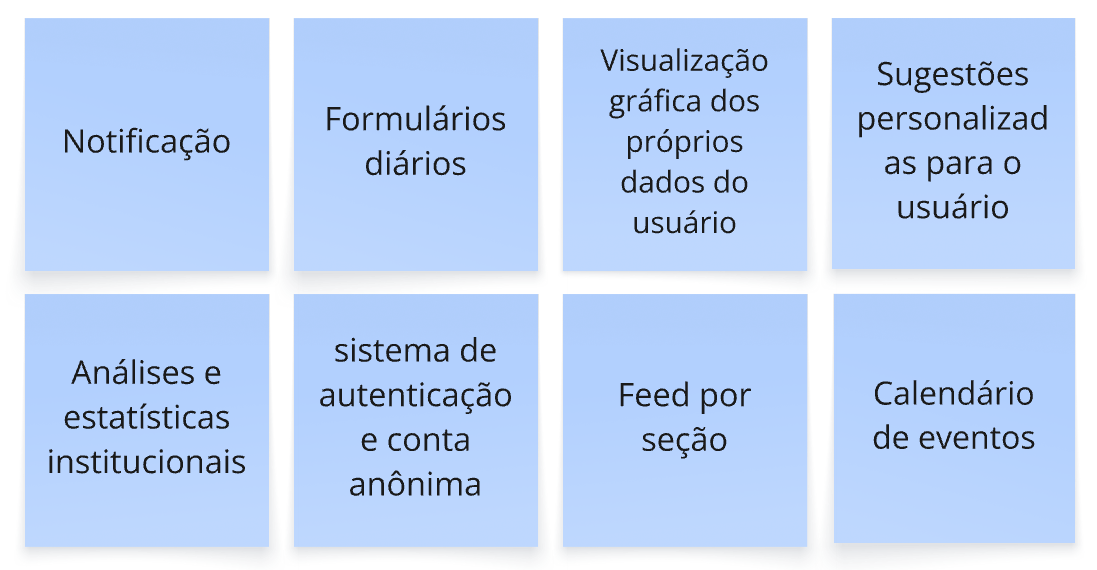
\includegraphics[width=1\textwidth]{figuras/lean/brainstorming_v2.png}
    \par
    Fonte: autoria própria.
    \par
    \label{brainstormingfunc}
\end{figure}

\section{Revisão (Técnica, de Negócio e Experiência do Usuário)}

A revisão técnica, de negócio e de experiência do usuário (UX) tem como objetivo avaliar as funcionalidades levantadas durante o \textit{brainstorming}, classificando-as com base em três critérios principais: valor de negócio, esforço técnico e impacto na experiência do usuário \cite{caroli2017lean}.

\begin{figure}[H]
    \centering
    \caption{Classificação de funcionalidades - Lean Inception.}
    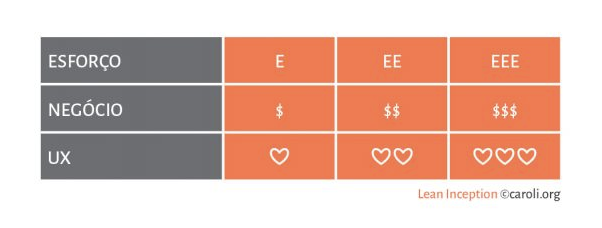
\includegraphics[width=0.8\textwidth]{figuras/lean/escalaesforco.png}
    \par
    Fonte: \citeonline{caroli2017lean}.
    \par
    \label{esforcolean}
\end{figure}

Em seguida, com base na classificação das funcionalidades, é utilizado o Gráfico do Semáforo, cujo objetivo principal é avaliar o nível de confiança da equipe de desenvolvimento em relação às tarefas propostas. Esse gráfico auxilia na análise da clareza sobre o que deve ser feito versus como deve ser feito \cite{caroli2017lean}.

%Sendo assim, as funcionalidades são distribuídas em zonas coloridas: itens posicionados na zona verde indicam alto nível de confiança e clareza; já as zonas vermelha devem ser evitadas e itens em zonas críticas devem ser excluídos do escopo \cite{caroli2017lean}.

%\begin{figure}[H]
%    \centering
%    \caption{Gráfico do Semáforo.}
%    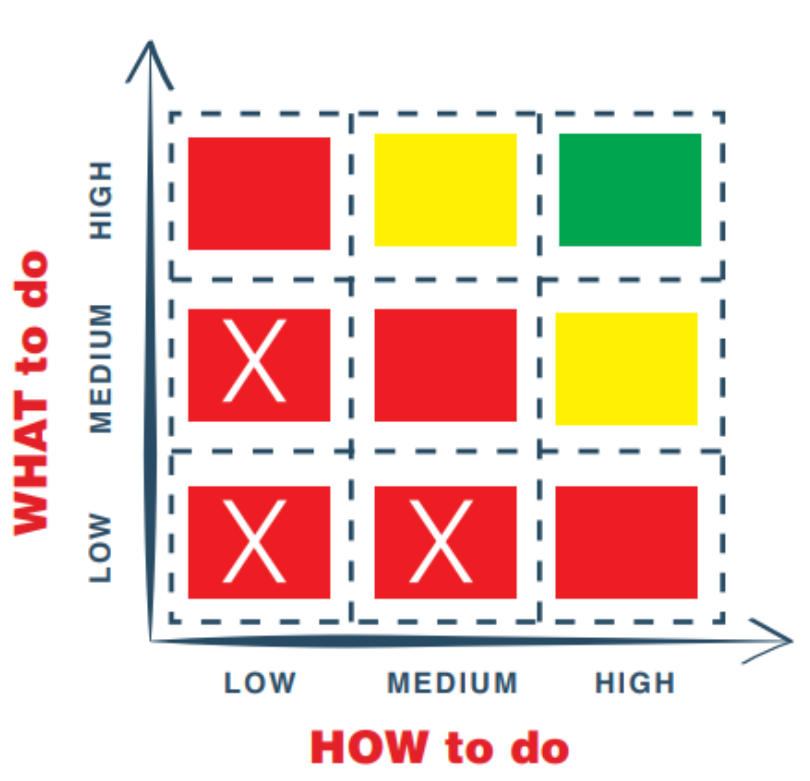
\includegraphics[width=0.5\textwidth]{figuras/revisaolean.png}
%    \par
%    Fonte: \citeonline{caroli2017lean}.
%    \par
%    \label{corlean}
%\end{figure}

Por meio desta etapa, as funcionalidades levantadas durante o \textit{Brainstorming} de Funcionalidades foram avaliadas quanto ao seu valor de negócio, esforço técnico e impacto na experiência do usuário (UX). A Figura~\ref{revisaolean} apresenta o resultado da revisão realizada para o projeto.

\begin{figure}[H]
    \centering
    \caption{Revisão das funcionalidades propostas (Seed).}
    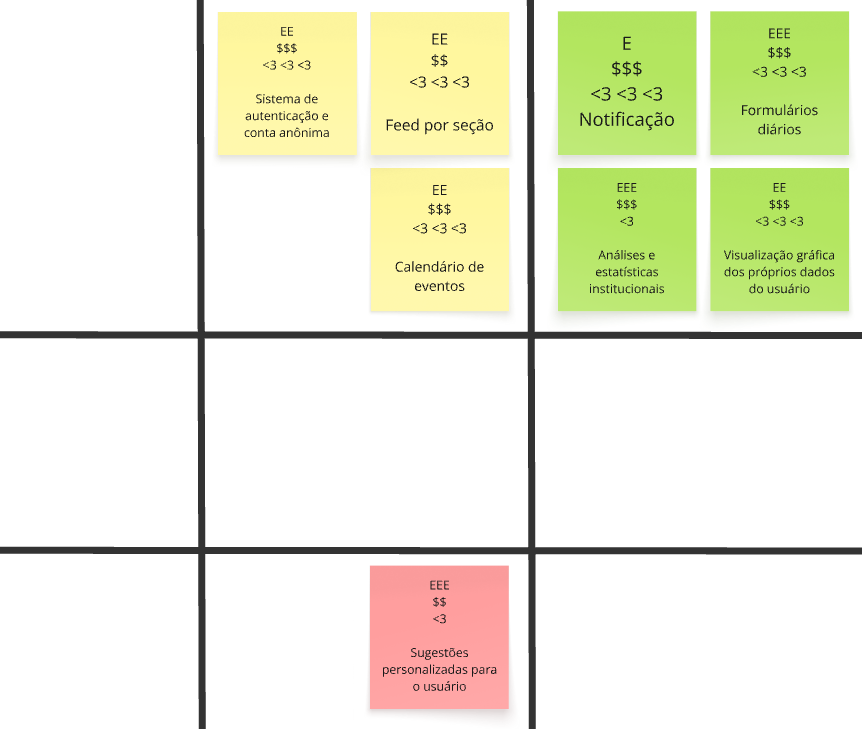
\includegraphics[width=1\textwidth]{figuras/lean/semafaro.png}
    \par
    Fonte: autoria própria com base em \citeonline{caroli2017lean}.
    \par
    \label{revisaolean}
\end{figure}

\section{Sequenciador}

%O sequenciador tem como objetivo organizar as funcionalidades em ondas, de forma a distribuir o trabalho progressivamente e evitar a sobrecarga da equipe de desenvolvimento. De acordo com \citeonline{caroli2017lean}, cada onda deve seguir alguns critérios para garantir equilíbrio entre valor entregue, esforço técnico e viabilidade:
%
%\begin{enumerate}
%    \item Cada onda deve conter, no máximo, três cartões;
%
%    \item Não é permitido que todos os cartões sejam classificados como vermelhos ou amarelos;
%
%    \item Cada onda pode conter, no máximo, um cartão vermelho;
%
%    \item A soma dos esforços técnicos não deve ultrapassar 5;
%
%    \item A soma dos valores de negócio e de experiência do usuário (UX) não deve ser inferior a 4 em cada critério;
%
%    \item Cartões com dependência entre si devem ser alocados em ondas distintas.
%\end{enumerate}
%
%Com base nesses critérios, a Figura~\ref{sequenciadorlean} apresenta o sequenciador elaborado para o projeto.

O sequenciador tem como objetivo organizar as funcionalidades em ondas, de forma a distribuir o trabalho progressivamente e evitar a sobrecarga da equipe de desenvolvimento \cite{caroli2017lean}. A Figura~\ref{sequenciadorlean} apresenta o sequenciador elaborado para o projeto.

\begin{figure}[H]
    \centering
    \caption{Sequenciador (Seed).}
    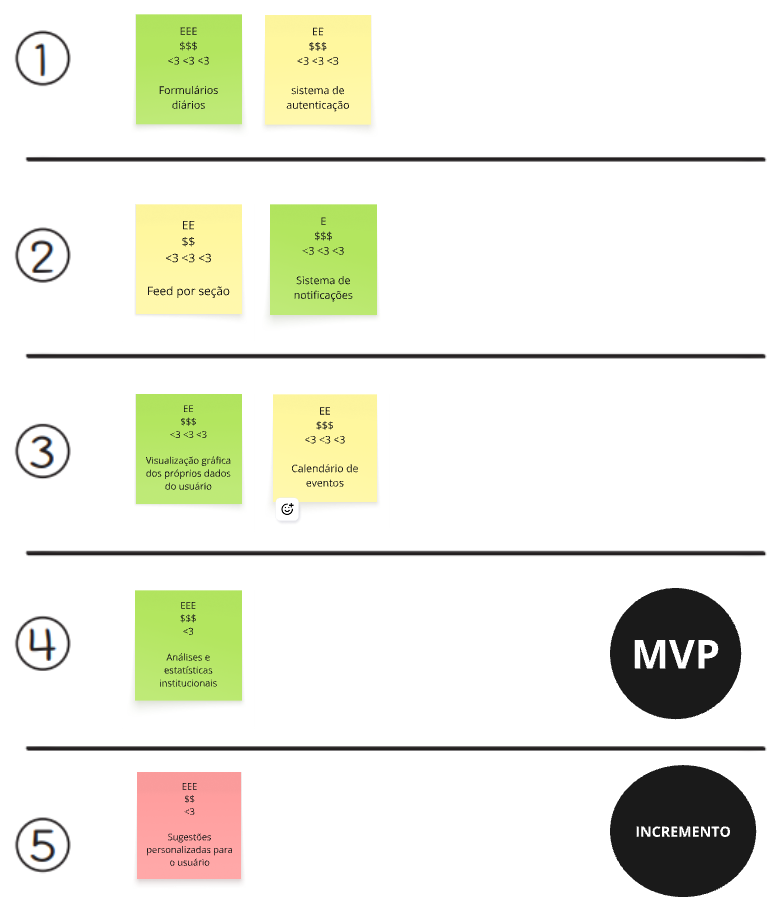
\includegraphics[width=0.7\textwidth]{figuras/lean/sequenciador}
    \par
    Fonte: autoria própria com base em \citeonline{caroli2017lean}.
    \par
    \label{sequenciadorlean}
\end{figure}

\section{Canvas MVP}

Ao final da Lean Inception, é elaborado o Canvas MVP, que consolida as principais definições do produto mínimo viável em sete blocos estruturados \cite{caroli2017lean}. Esses blocos são:

\begin{enumerate}
    \item Proposta do MVP;
    \item Personas Segmentadas;
    \item Jornadas;
    \item Funcionalidades;
    \item Resultado esperado;
    \item Métricas para validas as hipóteses de négocio;
    \item Custos e cronograma.
\end{enumerate}

A Figura~\ref{canvamvp} representa o produto final gerado a partir da aplicação da metodologia Lean Inception, reunindo as informações essenciais para a construção e validação do MVP.

\begin{figure}[H]
    \centering
    \caption{Canvas MVP (Seed).}
    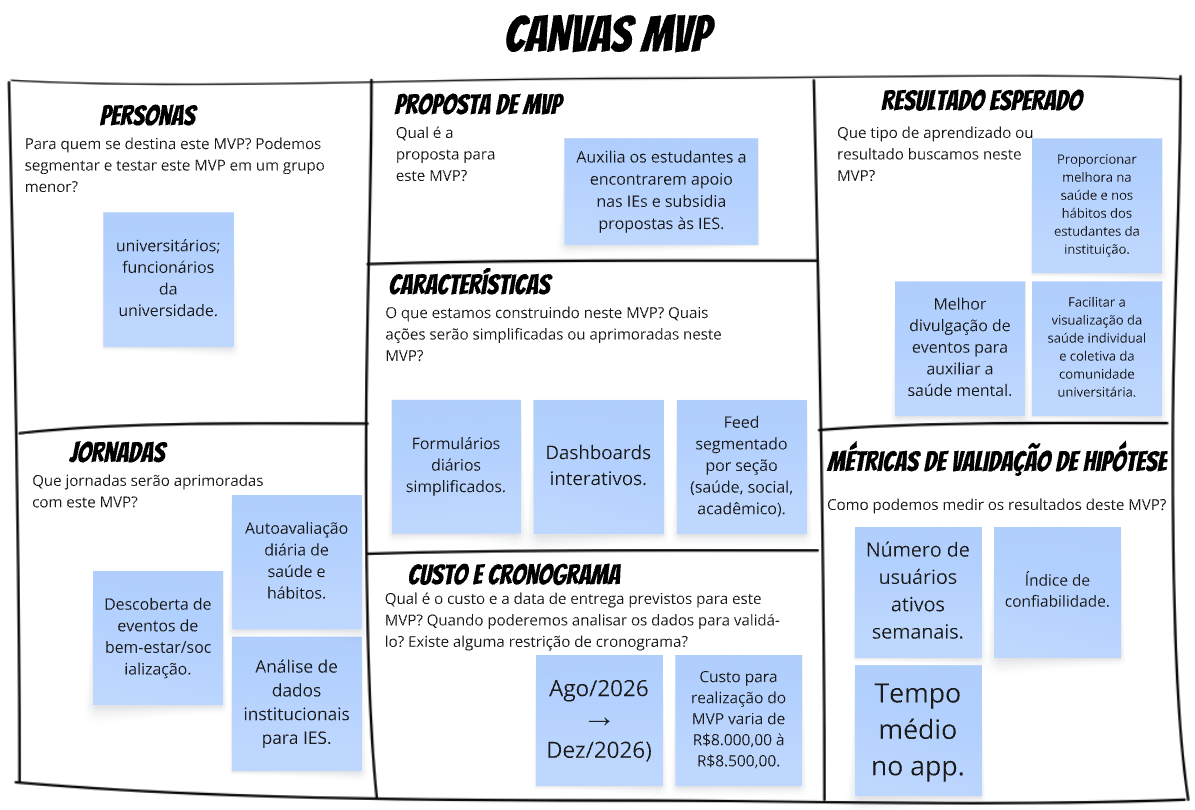
\includegraphics[width=1\textwidth]{figuras/lean/mvpcanvas}
    \par
    Fonte: autoria própria com base em \citeonline{caroli2017lean}.
    \par
    \label{canvamvp}
\end{figure}